\documentclass[a4paper]{article}
\usepackage[utf8]{inputenc} % Skal passe til editorens indstillinger
\usepackage[english]{babel} % danske overskrifter


\newcommand{\name}{Carsten Nielsen}
%\newcommand{\stnumber}{s123369, s123161, s123821}
\newcommand{\course}{INI 404 Neuromorphic Engineering~I}
\newcommand{\university}{University of Zürich}
\newcommand{\studyline}{Institute of Neuroinformatics}
\newcommand{\assignment}{Lab 8 Post-Lab}
\renewcommand{\date}{\today} %If another date, than that of today is desiered


% Palatino for rm and math | Helvetica for ss | Courier for tt
\usepackage{mathpazo} % math & rm
\linespread{1.05}        % Palatino needs more leading (space between lines)
\usepackage{palatino} % tt
\normalfont
\usepackage[T1]{fontenc}
\usepackage[english]{babel}

\usepackage{graphicx}%allerese hentet % indsættelse af billeder
\usepackage{epstopdf} %Tilfj "--enable-write18" i argumentet for LaTex build. Dette vil konvertere .eps figurer til pdf-format
\graphicspath{{./picture/}} % stivej til bibliotek med figurer
\usepackage{subcaption} %Til gruppering af figurer
\usepackage{amsmath} %matpakke
\usepackage{amsfonts} %
\usepackage{amssymb} %
\usepackage{steinmetz} % flere matematik symboler
\usepackage{polynom} %for displaying polynom division
\usepackage{mathtools} % matematik - understøtter muligheden for at bruge \eqref{}
\usepackage{float}
\usepackage{placeins}
\usepackage{hhline}

%
\usepackage[usenames,dvipsnames]{xcolor}
\usepackage[compact,explicit]{titlesec}% http://ctan.org/pkg/titlesec
%
\usepackage[europeanresistors]{circuitikz}
\usepackage{pgfplots}
\usepgfplotslibrary{patchplots}
\pgfplotsset{compat=1.11}

%---------%
%Easy edit%
%---------%

%Section formating. arg1 is supplied when making section
\newcommand\presectionnumber[1]{~~}
\newcommand\postsectionnumber[1]{}
\newcommand\midlesection[1]{#1}
\newcommand\sectionnum[1]{\arabic{#1}}
\newcommand\subsectionnum[1]{\arabic{#1}}
\newcommand\subsubsectionnum[1]{\alph{#1}}



%------------%
%setion setup%
%------------%
\renewcommand\thesection{Opgave~\sectionnum{section}} %pas p�, kun i matematik
\renewcommand\thesubsection{\thesection,~\subsectionnum{subsection}}
\definecolor{MagRed}{RGB}{190,40,15}
\definecolor{MathGreen}{RGB}{82,164,0}

\titleformat{\section}{\normalfont\sffamily\large\bfseries\color{MathGreen}}{}{0pt}{|\kern-0.15ex|\kern-0.15ex|\kern-0.15ex|\presectionnumber{#1}\sectionnum{section}\postsectionnumber{#1}\qquad\quad\midlesection{#1}\label{sec:\sectionnum{section}}}
\titleformat{\subsection}[runin]{\large\bfseries}{}{10pt}{\sectionnum{section}.\subsectionnum{subsection})~#1\label{sec:\sectionnum{section}.\subsectionnum{subsection}}}
\titleformat{\subsubsection}[runin]{\itshape}{}{0pt}{\subsectionnum{subsection},\subsubsectionnum{subsection}~#1\label{sec:\sectionnum{section}.\subsectionnum{subsection}.\subsubsectionnum{subsubsection}}}
%\titleformat{\subsubsection}{\bfseries}{}{0pt}{\alph{subsection}.\arabic{subsubsection})\qquad\quad#1\label{\arabic{section}\alph{subsection}\arabic{subsubsection}}}

%----------%
%page setup%
%----------%
\textwidth = 400pt
\marginparwidth = 86pt
\hoffset = -25pt
\voffset= -30pt
\textheight = 670pt

%--------%
%hyperref%
%--------%
\newcommand{\HRule}{\rule{\linewidth}{0.5mm}}
\usepackage{fancyhdr}
\usepackage[plainpages=false,pdfpagelabels,pageanchor=false]{hyperref} % aktive links
\hypersetup{%
  pdfauthor={\name},
  pdftitle={\assignment},
  pdfsubject={\course} }
%\usepackage{memhfixc}% rettelser til hyperref

%-------------%
%Headder setup%
%-------------%
\fancyhf{} % tom header/footer
\fancyhfoffset{20pt}
\fancyhfoffset{20pt}
\fancyhead[OL]{\name \\ INI 404}
\fancyhead[OC]{Date \\ \date}
\fancyhead[OR]{\university\\ \studyline}
\fancyfoot[FL]{}
\fancyfoot[FC]{\thepage}
\fancyfoot[FR]{}
\renewcommand{\headrulewidth}{0.4pt}
\renewcommand{\footrulewidth}{0.4pt}
\headsep = 35pt
\pagestyle{fancy}
 % style setup

%Listings%
\usepackage{listingsutf8}
\usepackage[framed,numbered]{matlab-prettifier}


%setup listings
\lstset{language=Matlab,
  extendedchars=true,
  language=Octave,                % the language of the code
  basicstyle=\ttfamily\footnotesize,           % the size of the fonts that are
  % used for the code
  numbers=left,                   % where to put the line-numbers
  numberstyle=\tiny\color{gray},  % the style that is used for the line-numbers
  stepnumber=2,                   % the step between two line-numbers. If it's 1, each line 
                                  % will be numbered
  numbersep=5pt,                  % how far the line-numbers are from the code
  backgroundcolor=\color{white},      % choose the background color. You must add \usepackage{color}
  showspaces=false,               % show spaces adding particular underscores
  showstringspaces=false,         % underline spaces within strings
  showtabs=false,                 % show tabs within strings adding particular underscores
  frame=single,                   % adds a frame around the code
  rulecolor=\color{black},        % if not set, the frame-color may be changed on line-breaks within not-black text (e.g. comments (green here))
  tabsize=4,                      % sets default tabsize to 2 spaces
  captionpos=b,                   % sets the caption-position to bottom
  breaklines=true,                % sets automatic line breaking
  breakatwhitespace=false,        % sets if automatic breaks should only happen at whitespace
  title=\lstname,                   % show the filename of files included with \lstinputlisting;
                                  % also try caption instead of title
  %keywordstyle=\color{blue},          % keyword style
  %commentstyle=\color{dkgreen},       % comment style
  %stringstyle=\color{mauve},         % string literal style
  escapeinside={\%*}{*)},            % if you want to add LaTeX within your code
  morekeywords={*,...},              % if you want to add more keywords to the set
  deletekeywords={...}              % if you want to delete keywords from the given language
}
\lstset{literate=
  {á}{{\'a}}1 {é}{{\'e}}1 {í}{{\'i}}1 {ó}{{\'o}}1 {ú}{{\'u}}1
  {Á}{{\'A}}1 {É}{{\'E}}1 {Í}{{\'I}}1 {Ó}{{\'O}}1 {Ú}{{\'U}}1
  {à}{{\`a}}1 {è}{{\`e}}1 {ì}{{\`i}}1 {ò}{{\`o}}1 {ù}{{\`u}}1
  {À}{{\`A}}1 {È}{{\'E}}1 {Ì}{{\`I}}1 {Ò}{{\`O}}1 {Ù}{{\`U}}1
  {ä}{{\"a}}1 {ë}{{\"e}}1 {ï}{{\"i}}1 {ö}{{\"o}}1 {ü}{{\"u}}1
  {Ä}{{\"A}}1 {Ë}{{\"E}}1 {Ï}{{\"I}}1 {Ö}{{\"O}}1 {Ü}{{\"U}}1
  {â}{{\^a}}1 {ê}{{\^e}}1 {î}{{\^i}}1 {ô}{{\^o}}1 {û}{{\^u}}1
  {Â}{{\^A}}1 {Ê}{{\^E}}1 {Î}{{\^I}}1 {Ô}{{\^O}}1 {Û}{{\^U}}1
  {œ}{{\oe}}1 {Œ}{{\OE}}1 {æ}{{\ae}}1 {Æ}{{\AE}}1 {ß}{{\ss}}1
  {ç}{{\c c}}1 {Ç}{{\c C}}1 {ø}{{\o}}1 {å}{{\r a}}1 {Å}{{\r A}}1
  {€}{{\EUR}}1 {£}{{\pounds}}1
}

 \lstloadlanguages{% Check Dokumentation for further languages ...
         %[Visual]Basic
         %Pascal
         %C
         %C++
         %XML
         %HTML
         %Java
         %VHDL
         Matlab
 }
 %Listings slut%









%Matematik hurtige ting
%fed
\renewcommand\vec[1]{\mathbf{#1}}
\newcommand\matr[3]{{}_{#2}\mathbf{#1}{}_{#3}}
\newcommand\facit[1]{\underline{\underline{#1}}}
%\renewcommand\d[3]{\frac{\mbox{d}^{#3}#1(#2)}{\mbox{d}#2^{#3}}}
%underline
%\renewcommand\vec[1]{\underline{#1}}
%\newcommand\matr[3]{{}_{#2}\underline{\underline{#1}}{}_{#3}}

\renewcommand\matrix[4]{ %{alignment}{to space}{from space}{matrix}
{\vphantom{\left[\begin{array}{#1}#4\end{array}\right]}}_{#2}\kern-0.5ex
\left[\begin{array}{#1}
#4
\end{array}\right]_{#3}
}
\newcommand\e[0]{\mbox{e}}
\newcommand\E[1]{\cdot 10^{#1}}
\newcommand\im[0]{i}

\newcommand\Jaco{\mbox{Jacobi}}
\newcommand\del[2]{\frac{\partial {#1}}{\partial {#2}}}
\newcommand\abs[1]{\left| {#1} \right|}
\newcommand\stdfig[4]{ %width,img,cap,lab
\begin{figure}[H]
\centering
\includegraphics[width={#1}\textwidth]{#2}
\caption{#3}
\label{#4}
\end{figure}
}
\newcommand\stdfignoscale[3]{ %img,cap,lab
\begin{figure}[H]
\centering
\includegraphics{#1}
\caption{#2}
\label{#3}
\end{figure}
}
\newcommand\diff{\dot}
\newcommand\ddiff{\ddot}
\newcommand\dddiff{\dddot}
\newcommand\ddddiff{\ddddot}






% How to make ref to books or urls in bib
%\citetitle[fx: page 1]{name of ref in bib}


\tikzset{rrail/.style={rground,yscale=-1}}
\newcommand{\reffig}[1]{Fig.~\ref{#1}}

\begin{document}
\begin{titlepage}
\centering \parindent=0pt

\vspace*{\stretch{1}} \HRule\\[1cm]\Huge
\course\\[0.7cm]
\large \assignment\\[1cm]
\HRule\\[4cm]  
%\includegraphics[width=6cm]{picture}\\ Use this if you want a picture on the frontpage
\name\\
%\stnumber
TAs: Ning Quiao, Chenghan Li

\vspace*{\stretch{2}} \normalsize %

\begin{center}
	\date 
\end{center}
\vspace*{\stretch{2}} \normalsize
\begin{flushright}
%\includegraphics[width=6cm]{./dtu.eps}\\
\end{flushright}
\end{titlepage}

\newpage
\begin{figure}
    \center
    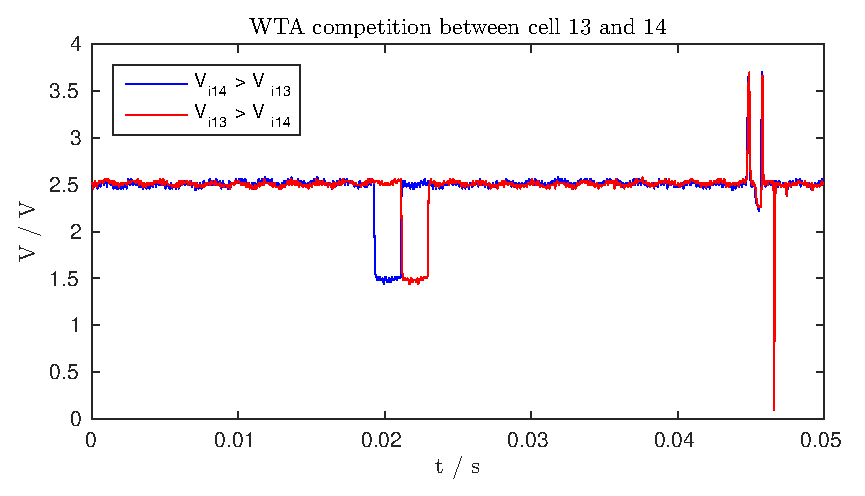
\includegraphics{ex1.eps}
    \caption{Competition between cell 13 and 14 in the WTA network. When the input current to cell 13 is larger than that to cell 14, cell 13 produces all the output current, and
        vice-verse for cell 14. 
    The artefacts on the right hand side occur when scanning cell 26 and 1.}
    \label{fig:ex1}
\end{figure}
\section{Experiment 1: Observing Behaviour of the WTA}
We connected the sync input to channel 2 of the oscilloscope and used triggered off of it with a holdoff of 48ms in order to trigger once on every pass through the
scan chain. This way we were able to obtain the waveforms shown in Fig.~\ref{fig:ex1} where the waveform for a winning cell 13 is overlaid with a winning cell 14.
The cell with the highest input voltage loses because the input voltage is applied to the gate of a pFET, meaning that a higher voltage leads to a lower input current.
We cannot explain the glitches observable to the right. However, they interestingly appear at the border cells numbered 26 and 1.
\begin{figure}
    \center
    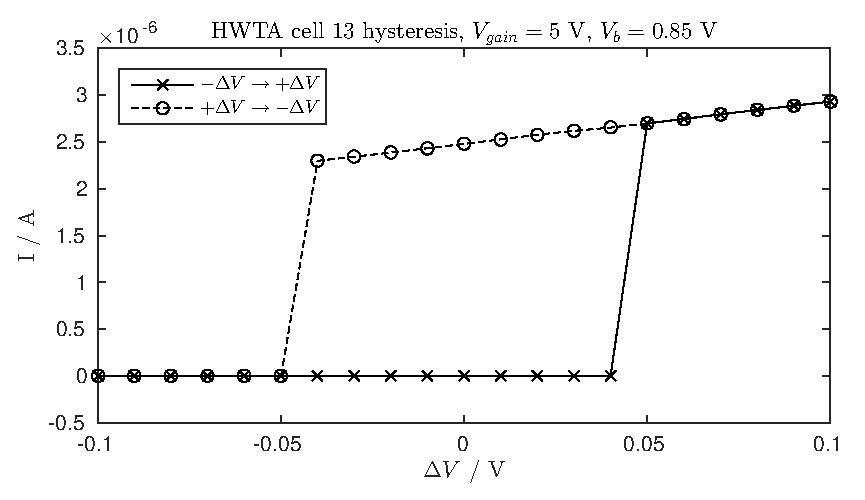
\includegraphics{ex2-1.eps}
    \caption{Hysteresis in the HWTA circuit. \(\Delta V\) starts out negative and then moves to positive values before going back to negative values.
    \(V_{gain}=5\) V which results in a small hysteretic loop.}
    \label{fig:ex2-1}
\end{figure}
\section{Experiment 2: Two Cell Competition}
We measured the current through cell 13 as a function of differential voltage between cell 13 and 14 using 4.2 V as the bias input voltage.
Fig.~\ref{fig:ex2-1} shows the current for \(V_{gain}=5\) V, Fig.~\ref{fig:ex2-2} for \(V_{gain}=4.5\) V and Fig.~\ref{fig:ex2-3} for \(V_{gain}=4\) V.
\(V_b\) was kept at 0.85 V throughout the experiment.
\begin{figure}
    \center
    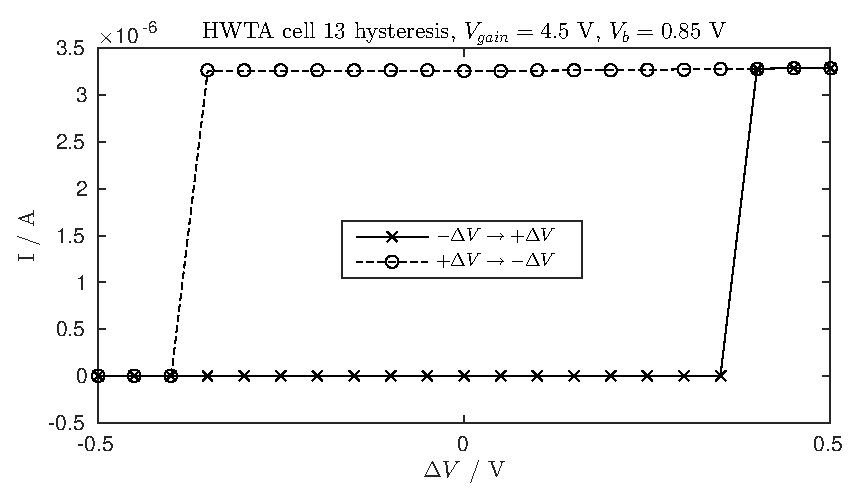
\includegraphics{ex2-2.eps}
    \caption{Hysteresis in the HWTA circuit for \(V_{gain}=4.5\) V. Here the hysteretic loop is much larger than for \(V_{gain} = 5\) V.}
    \label{fig:ex2-2}
\end{figure}
\begin{figure}
    \center
    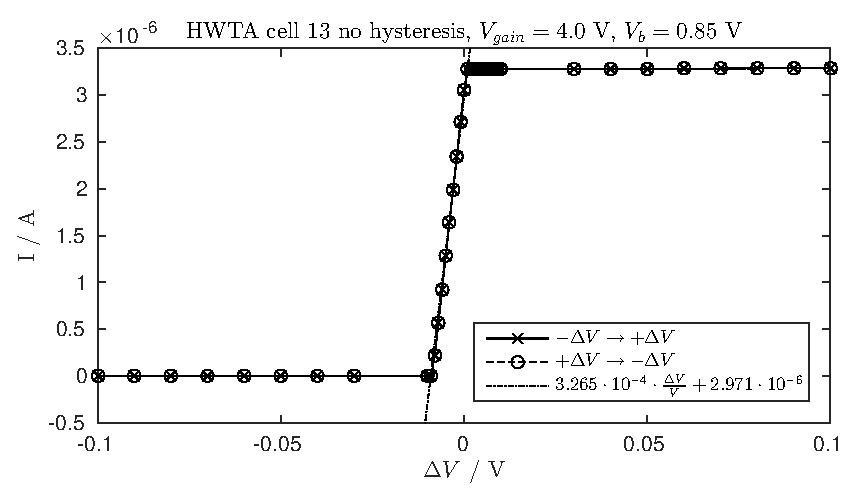
\includegraphics{ex2-3.eps}
    \caption{HWTA current through cell 13 with \(V_{gain}=4.0\) V. No hysteresis is observed with this gain voltage. The gain of the linear part of the slope is
    3062.}
    \label{fig:ex2-3}
\end{figure}

Interestingly, the output current does not immediately max out for the case where \(V_{gain}=5 \) V, but instead continues to rise linearly
as \(\Delta V\) is increased for the range that we measured. The width of the hysteresis loop is also larger for \(V_{gain}=4.5\) V which should not happen.
The gain voltage parameter is the source voltage to the pMOS transistor which delivers the excitatory feedback to the winning node. The larger this value becomes,
the wider the hysteresis loop should become. This is because the excitatory feedback acts as a secondary input current which aids the winning node in succeeding and keeping
the winning spot.

When the gain voltage parameter is decreased sufficiently such that the width of the hysteresis loop effectively disappears, we are left with the standard WTA circuit
which has a high current gain in a very small region of operation as the node switches from losing to winning or vice-versa. The gain of the high gain part of the
curve is 3062. This is much less than the number we derived in the pre-lab where we assumed \(\kappa = 0.8\) and \(V_E \simeq 450\) V. Of course, this Early voltage is
much too large as we measured in a previous lab that the Early voltages for the 16 micron transistors was around 140 V. With a gain of 3062, the output transistors
in the WTA circuit have an Early voltage of aroun 100 volts assuming \(\kappa = 0.8\) and \(U_T = 26\) mV.
\end{document}
